\documentclass{article}

% \usepackage{fullpage}
\usepackage{titling}
\usepackage{amsmath}
\usepackage{graphicx}
\graphicspath{ {./resources/} }
\usepackage{etoolbox}
\patchcmd{\thebibliography}{\section*{\refname}}{}{}{}

\setlength{\parindent}{0pt}
\addtolength{\oddsidemargin}{-.875in}
\addtolength{\evensidemargin}{-.875in}
\addtolength{\textwidth}{1.75in}

\addtolength{\topmargin}{-.375in}
\addtolength{\textheight}{1in}

\title{CS3243 Tetris Project}
\author{Varun Gupta \and Gao Bo \and Advay Pal \and Chang Chu-Ming \and Herbert Ilhan Tanujaya}
\date{13-04-2017}

\begin{document}
	\maketitle
	\thispagestyle{empty}
	\vspace{5mm}

    \section{Introduction}
    Tetris is likely one of the world's most famous and popular games.
    In this report, we describe how we devise an agent to play the game of Tetris.
    We use an agent that greedily picks the best possible next state from a given state,
    by using a heuristic function to approximate the value of a state. To train our heuristic
    function, we use a novel algorithm that is a combination of the well known Genetic Algorithm (GA)
    and Particle Swarm Algorithm (PSO). Our agent manages to clear \textbf{TODO} million lines on average with a max
    of \textbf{TODO} million lines, demonstrating that our algorithm is effective.

    \section{Agent Strategy}
	Our agent uses a linear weighted sum of features as the heuristic function for
	a given state. Here, a state is defined by the field of the board. Given a
	state and a piece, the agent computes the heuristic value for all possible next
	states, and then greedily picks the next state with the maximum heuristic
	value. In other words, the next state is chosen by \[ \max_{s' \in N(s, p)}
	\left\{ \sum w_i f_i(s') \right\}, \] where $s$ is the original state, $N(s,
	p)$ is the set of all possible next states from $s$ and a piece $p$, $f_i(s')$
	is the score of feature $i$ on state $s'$ and $w_i$ is the weight of feature
	$i$.

    \section{Features}
    We used the following features for our heuristic function:
    \begin{itemize}
        \item Altitude Difference ($AltD$): The difference between the height of the highest
        column and the height of the lowest column
		\item Column Transition ($ColT$): Number of adjacent squares in a column with opposite parity (where parity is defined as either full or empty)
		\item Deepest Well ($DW$): Height of the lowest column
        \item Height ($ColH$): Height of the highest column
		\item Number of Columns With Holes ($CwH$): The number of columns with holes, where a hole
		is defined as an empty square directly beneath a filled square
        \item Number of Holes ($NHole$): Number of holes in the entire board
        \item Number of Wells ($NWell$): The number of columns that have a height less than that of the 2
        adjacent columns
		\item Rows Cleared ($RC$): The number of rows cleared for that particular move
		\item Row Transition ($RowT$): Number of adjacent squares in a row with opposite parity (where parity is defined as either full or empty)
        \item Total Column Height ($TColH$): The sum of the heights of all the columns
        \item Total Column Height Difference ($TColHD$): The sum of the difference of heights between adjacent columns
        \item Weighted Block ($WB$): Sum of value of every square, where a square's value is equal to
		the row it is in (numbered from the bottom)
        \item Well Sum ($WellS$): Using the same definition of wells as above, this sums up
		the depth of every well
    \end{itemize}

    While running our training algorithms, we noticed that some features were more
	important than others. In particular, the algorithm assigned highly negative
	weights to Column Transition and Well Sum, while assigning highly positive
	weights to Number of Wells. This was slightly unexpected as we thought that
	Rows Cleared would have the largest positive weights, to predispose the algorithm
	towards clearing more rows. However, the weight for this heuristic varied wildly
	between positive and negative, indicating that perhaps sometimes the algorithm
	preferred to not greedily pick moves that were clearing rows, but rather chose
	to maintain an even surface at the top.

    \section{Our Algorithm}

    Our algorithm consists of a combination of a genetic algorithm and particle swarm
	optimization (PSO) algorithm. We run both of these algorithms on different ‘islands’
	with population sizes of a 100 each. Each member of our population is a heuristic (set of weights).
	The key idea is that both of the algorithms run individually, but after each generation, we
	copy the 10 best heuristics on each island to the other one.\\
	\newline
	We will first describe the working principle
	of the Genetic and the PSO algorithms. Subsequently, we will
	discuss the rationale behind why we chose to juxtapose these two different
	algorithms in our search for the best heuristic, as well as how we did so.\\

	Genetic algorithm\\
	For this algorithm, a crossover is done by taking two parent heuristics, and
	for every feature selecting the weight from one of the parents randomly. A
	mutation is defined as multiplying the current weight of a feature with
	a value normally distributed with a mean of 1 and a standard deviation of 1.\\
	Each generation of our genetic algorithm consists of the following sequence of steps
	\begin{enumerate}
		\item Evaluate fitness of each set of heuristics
		\item Keep top half of population and cross-over the rest
		\item Random mutation of each feature of crossed-over heuristics with
		probability 0.1
		\item Migrate 0.1 of the population to PSO island
	\end{enumerate}
	We keep the top half of the population to ensure that each set of heuristics
	that perform well will remain within the population. The mutation introduces
	some randomness to the genetic algorithm to avoid being trapped within a local
	maximum.\\

	PSO algorithm\\
	The PSO algorithm treats every heuristic as a point in 13-dimensional space.
	This is the position of the heuristic. Each heuristic also has a velocity,
	a vector in the 13-dimensional space, which is added to the position to get
	new population members.
	Each generation of our PSO algorithm consists of the following sequence of steps
	\begin{enumerate}
		\item Set velocity of each member to a linear weighted sum of the old velocity,
		the personal best of that member, and the global best
		\item Get new position of each member by adding its velocity to the current
		position
		\item Evaluate fitness of each set of heuristics
		\item Migration of a tenth of the population to PSO island
	\end{enumerate}
	For PSO, it is almost certain that every member of the population is mutated
	in every generation since weighted velocity is very unlikely to be 0.\\

	Rationale behind combination of algorithms\\
	We ran PSO and GA individually. In doing so, we realised that PSO was in general not doing
	very well, but that it sometimes made a leap and jumped by almost an order of magnitude
	in terms of lines cleared. On the other hand, Genetic seemed to keep getting
	better, but only quite slowly. From these experimental results, we hypothesised
	that Genetic may have been doing more of exploitation, finding the maximum in the local area,
	while PSO may have been doing more of exploration, looking for good solutions all over
	the search space. Hence we thought that perhaps if we combined the two,
	PSO could lead Genetic to better areas, which Genetic could then drill down into.
	This would allow us to achieve a more balanced trade-off between exploitation
	and exploration, which we hoped would make our algorithm more efficient.

	\section{Further Optimisation}
	The hyperparameters for both the genetic algorithm and the PSO algorithm need
	to be optimized for our integrated solution to learn at an optimal rate.
	Given limited time, we decided to focus our attention on the hyperparameters
	of the PSO algorithm. The rationale behind this is that while the genetic
	algorithm learns at a steady rate, the PSO algorithm tends to make large jumps
	in progress and can explore larger swaths of the search-space in a shorter
	time. We felt that if we successfully could optimize the PSO algorithm, it would be able to
	find a solution close to the global maximum and share this information with the genetic algorithm.
	The genetic algorithm would then refine the solution further.

	One of the issues that we observed is that even with the same set of hyperparameters,
	different initializations of random variables such as mutation can lead to
	different rates of learning. Thus, we ran multiple jobs in parallel and averaged
	their results to determine which set of hyperparameters work best.

	The hyperparameters of the PSO algorithm consist of $\rho_g$ and $\rho_p$, the constants
	which determine the effect of the global and personal bests on each iteration
	of velocity change; and $\omega$, the constant of inertia. Typically[CITE], $\rho_g$ and $\rho_p$ are both
	set to 2.0, which leaves $\omega$ to be optimized. A high $\omega$ will favour exploration,
	while a low $\omega$ will favour exploitation. Based on the observations of \cite{shi1998parameter}, we decided to first test values of $\omega$ between 1.2 to 0.6.
	While initializations with low $\omega$ generally performed better, the results were
	not conclusive. Thus, we decided that instead of a fixed $\omega$, we could vary it
	based on how close the population is to the global maximum. This is estimated
	by taking $\log_{10}$ of the average fitness scores of the population. The formula is as follows:

	\begin{center}
		$\omega = 1.2 - k(\log_{10}\text{(Average Fitness)} - 3)$
	\end{center}

	We tested different values of $k$ by running multiple jobs for an hour and comparing
 	the average of the fitness scores. Through experimentation, we found that the
	algorithm performs best when $k$ is 0.2. The experimental results are shown below.

	Note: The values below are taken across 5 instances with the same hyperparameters.\\

	\underline{Fixing and tuning $\omega$}\\
	Lower $\omega$ = more exploitation, worse maximum, better average\\
	Higher $\omega$ = more exploration, better maximum, worse average\\

	\begin{tabular}{ | c | c | c | }
		\hline
		$\omega$ & Maximum of Average Fitness & Average of Average fitness \\ \hline
		0.6 & 44807 & 30935 \\ \hline
		0.8 & 58192 & 27357 \\ \hline
		1.0 & 69375 & 26849 \\ \hline
		1.2 & 72743 & 20381 \\ \hline
	\end{tabular}\\[0.5em]

	\underline{Varying $\omega$ and tuning $k$}\\
	Higher $k$ = more varying $\omega$ = stronger transition from exploration to exploitation\\
	Lower $k$ = less varying $\omega$ = weaker transition from exploration to exploitation\\

	\begin{tabular}{ | c | c | c | }
		\hline
		$k$ & Maximum of Average Fitness & Average of Average fitness \\ \hline
		0.1 & 50260 & 32939 \\ \hline
		0.15 & 47115 & 30010 \\ \hline
		0.2 & 74838 & 38478 \\ \hline
	\end{tabular}

    \section{Experiments and Analysis}

	\subsection{Learning Perfomance}
	We ran our learning algorithm on nodes provided by the National Supercomputing Centre.
	The nodes we ran on had the following architecture specifications: E5-2690 v3 @ 2.60GHz.
	Using this, the results we obtained were:

	\begin{figure}[h]
		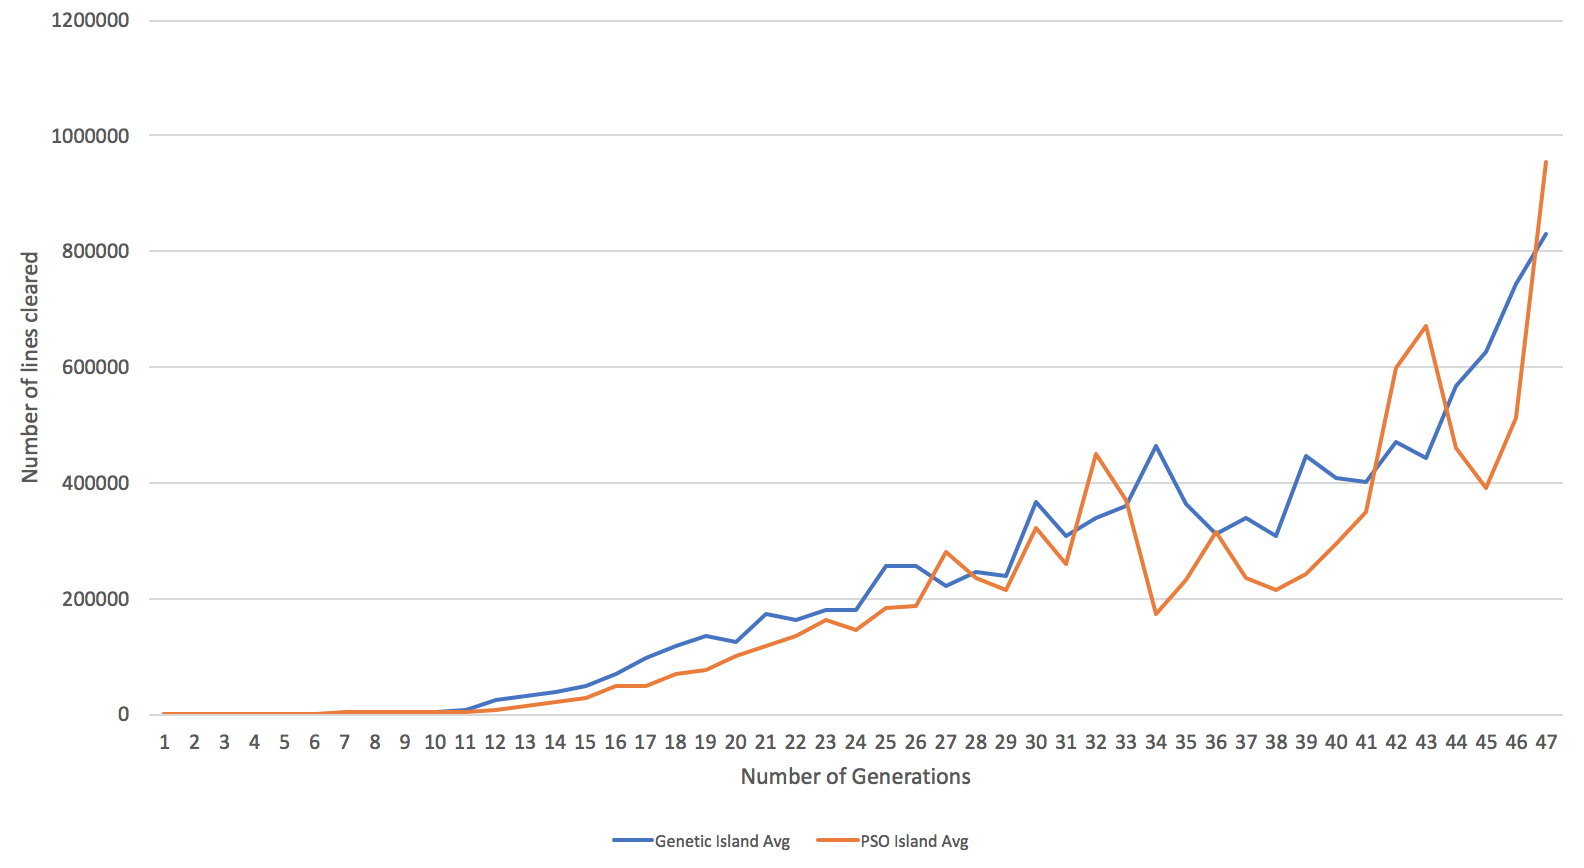
\includegraphics[scale=0.28]{learning/AlgoMax}
		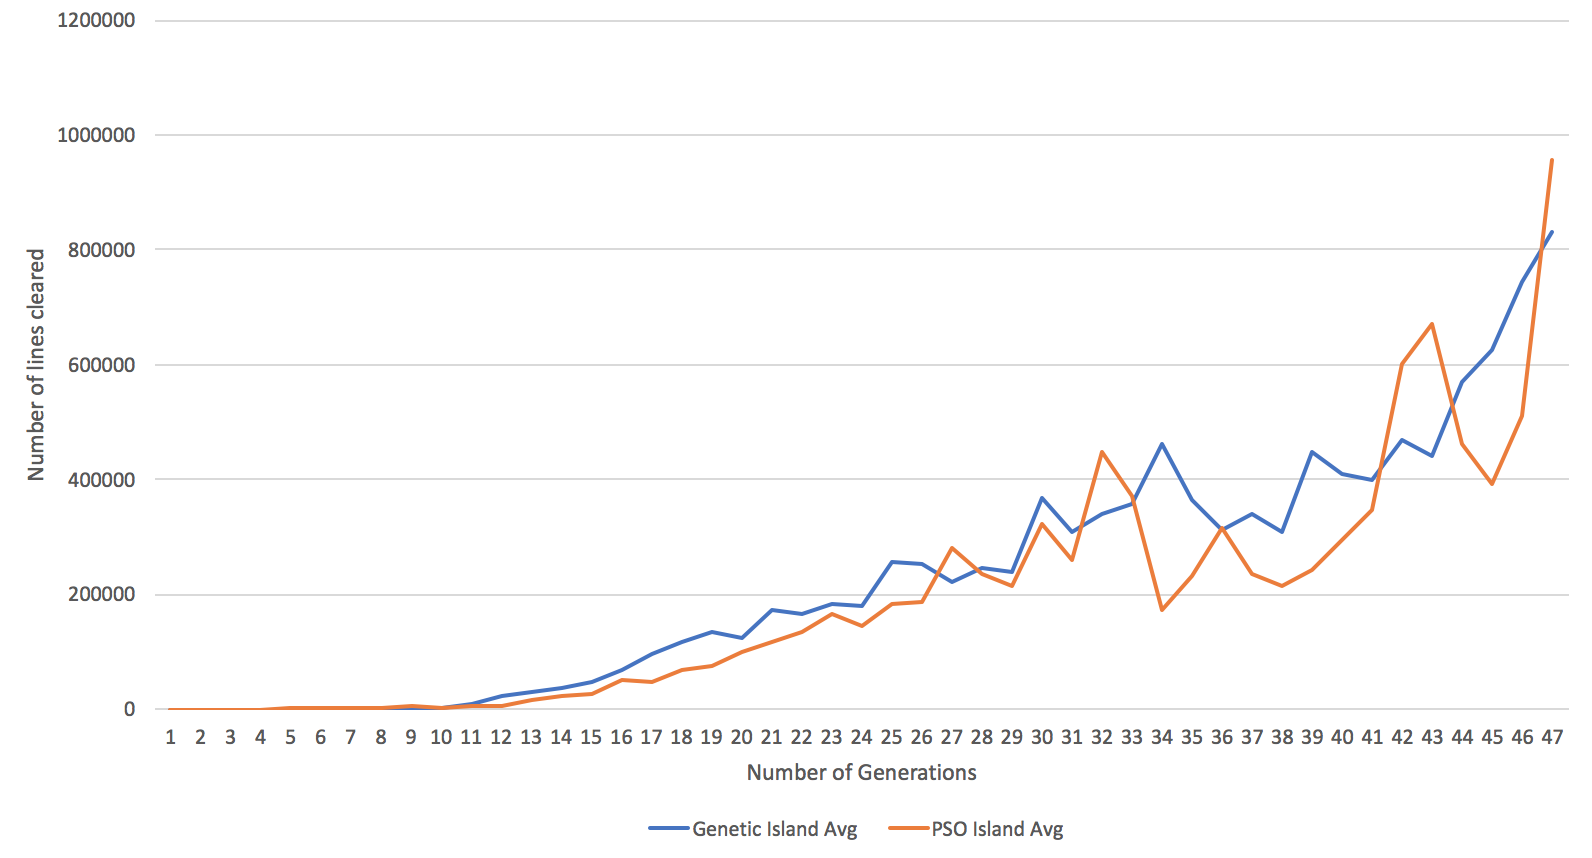
\includegraphics[scale=0.28]{learning/AlgoAvg}
		\centering
		\caption{Performance of the Learning Algorithm}
		\label{fig:learning}
	\end{figure}

	The first figure plots the number of lines cleared by the best heuristic in
	the Genetic and PSO islands over 47 generations, while the second figure plots
	the average number of lines cleared by the populations of the Genetic and PSO
	islands over the same generations. It can be seen that sometimes PSO leads the
	way in the first figure, producing a good heuristic that Genetic then builds
	upon. However, this is not always true, and in fact we did observe in other
	runs of the algorithm that sometimes Genetic also led the way.\\
	We also compared the results of our algorithm with Naive Genetic and Naive PSO
	(i.e. we ran them in isolation). The results obtained were:

	\begin{figure}[h]
		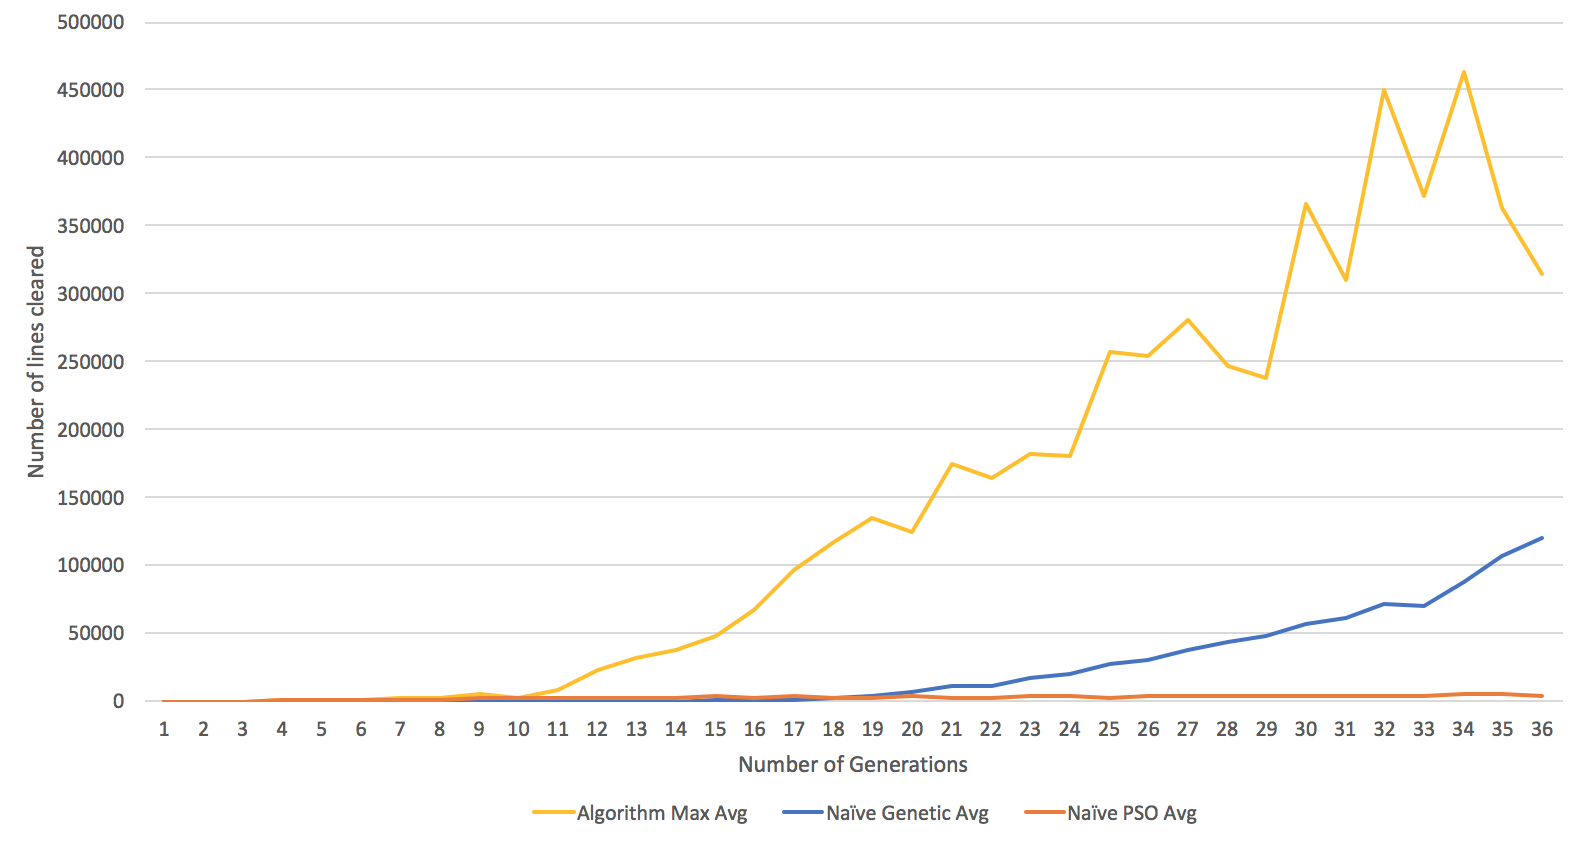
\includegraphics[scale=0.4]{learning/Naive}
		\centering
		\caption{Comparison of Learning Algorithm with Naive Genetic/PSO}
		\label{fig:naive}
	\end{figure}

	This figure plots the maximum of the average of Genetic and PSO islands for
	our learning algorithm, and compares it with the averages of Naive Genetic and
	Naive PSO. It can be seen that our algorithm performed far better, with PSO
	getting stuck at around 20 thousand lines cleared and Genetic rising very slowly.

	However, we can also observe from Figure \ref{fig:learning} that there is a large amount
	of variability in the results of the algorithm. One reason for this is the element
	of randomness in the algorithm itself, for example, in the mutation amount and threshold
	in Genetic and in the initial velocity imparted to a particle in PSO. There is
	a large amount of randomness in the game of tetris itself, as seen more clearly
	in the section analysing our agent's performance.

	Using a version of our algorithm that used 2 threads (one per island),
	we were able to get to a maximum of around 4 million lines cleared in
	around a day. Running a parallelised version (see below) we got to a maximum of
	around 18m in 10 hours.\\

	\subsection{Agent Performance}
	The best weights we obtained were:\\

	\begin{tabular}{ | c | c | c | c | c | c | c | c | c | c | c | c | c | }
		\hline
		$AltD$ & $ColT$ & $DW$ & $ColH$ & $CwH$ & $NHole$ & $NWell$ & $RC$ & $RowT$ & $TColH$ & $TColHD$ & $WB$ & $WellS$ \\ \hline
		0 & 0 & 0 & 0 & 0 & 0 & 0 & 0 & 0 & 0 & 0 & 0 & 0 \\ \hline
	\end{tabular}\\[0.25em]

	We ran the heuristic on \textbf{TODO} games, encapsulated in the following graph:\\

	\begin{figure}[h]
		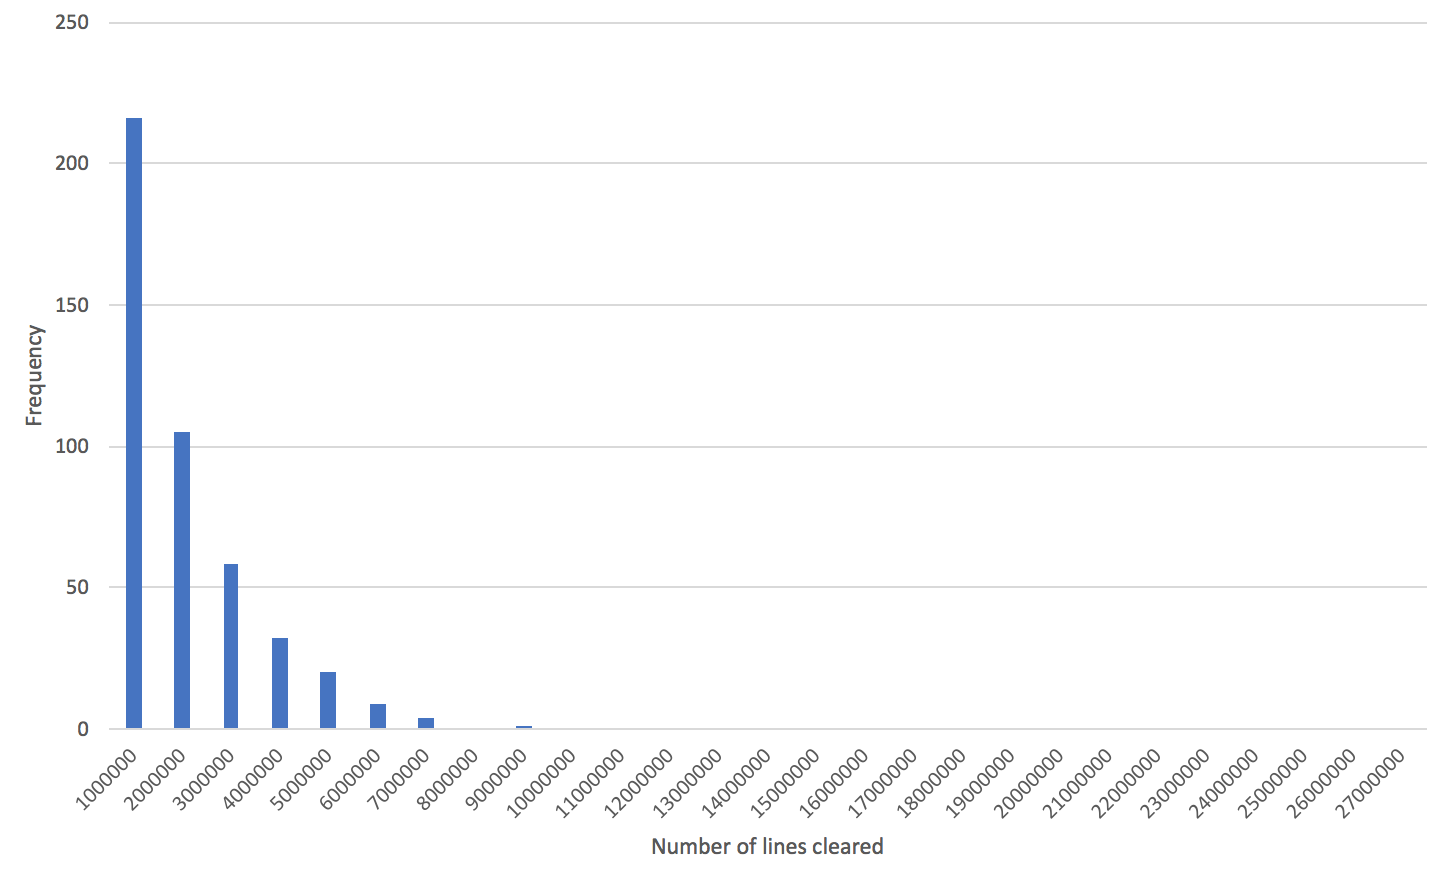
\includegraphics[scale=0.4]{heuristic/heuristic}
		\centering
		\caption{Performance of our Agent}
		\label{fig:agent}
	\end{figure}

	\vspace{-4mm}
	\begin{center}
		\begin{tabular}{ | c | c | c | }
			\hline
			Maximum & Minimum & Average \\ \hline
			0 & 0 & 0 \\ \hline
		\end{tabular}\\
	\end{center}

	As can be seen in Figure \ref{fig:agent}, there is a large variability in how
	well the heuristic performs, hitting a maximum of \textbf{TODO} and a minimum of \textbf{TODO}.
	This is likely because of the large randomisation within the game of tetris,
	with the sequences of pieces having a large impact on the performance. For example,
	a long sequence of $S$ and $Z$ pieces is impossible to get through successfully.

    \section{Scaling to Big Data}
	In order to scale to Big Data, we considered how our algorithm performed in the presence
	of multiple cores. We found that parallelising our algorithms through the use
	of multithreading lead to a linear speedup, demonstrating that our algorithm scaled very
	well in the presence of multiple cores. We attribute this to the fact that
	both Genetic Algorithms and PSO algorithms are embarassingly parallel, which
	is why we were able to achieve an optimal speedup quite easily.\\

	We parallelised our algorithm by running the PSO and Genetic islands on different cores,
	and further parallelised it by calculating the fitness of each population member on different cores.
	We did this as the major computational cost the algorithm was incurring came from
	the calculation of the fitness values, since that involved running entire tetris games.

	To demonstrate the effect of parallelisation, we recorded the speedup of our algorithm when run
	on multiple cores. We started both algorithms as two separate jobs on single machines
	in the NSCC cluster (which provide 12 cores each) at the same time, and allowed them to run for around 20
	hours before comparing the results. We used the total number of lines cleared
	in the entire time span as a rough estimate of the total amount of
	CPU time used. Our results showed that the single-threaded algorithm cleared
	a total of $158182993$ lines, while the multi-threaded version cleared a total
	of $1899941699$ lines. This shows that parallelisation provides a speedup of 12 times,
	which is optimal since each machine has 12 cores.

    \section{Conclusion}



    \section{References}
	\bibliographystyle{apalike}
	\bibliography{./resources/bibliography/references}


\end{document}
